\documentclass[a4paper,11pt]{book}
\usepackage[latin1]{inputenc}
\usepackage[T1]{fontenc}
\usepackage{epsfig}
\usepackage{url}
\usepackage{color}


% some tex code to generate both dvi and pdf files easily
\newif\ifpdf
\ifx\pdfoutput\undefined
    \pdffalse          % we are not running PDFLaTeX
\else
    \pdfoutput=1       % we are running PDFLaTeX
    \pdftrue
\fi
\ifpdf
    \usepackage[pdftex,
        colorlinks=true,
        urlcolor=rltblue,               % \href{...}{...}
        anchorcolor=rltbrightblue,
        filecolor=rltgreen,             % \href*{...}
        linkcolor=rltred,               % \ref{...} and \pageref{...}
        menucolor=webdarkblue,
        citecolor=webbrightgreen,
        pdftitle={A Short Introduction to Synergy/Change 4.3 Administration},
        pdfauthor={Boris Baldassari},
        pdfsubject={A Short Introduction to Synergy/Change 4.3 Administration},
        pdfkeywords={telelogic synergy change configuration management change},
        pagebackref,
        pdfpagemode=None,
        bookmarksopen=true]{hyperref}
    \pdfcompresslevel=9
    \usepackage{thumbpdf}
\else
    \usepackage[
        colorlinks=true,
        urlcolor=rltblue,               % \href{...}{...}
        anchorcolor=rltbrightblue,
        filecolor=rltgreen,             % \href*{...}
        linkcolor=rltred,               % \ref{...} and \pageref{...}
        menucolor=webdarkblue,
        citecolor=webbrightgreen]{hyperref}
    \usepackage{graphicx}
\fi


\definecolor{rltbrightred}{rgb}{1,0,0}
\definecolor{rltred}{rgb}{0.75,0,0}
\definecolor{rltdarkred}{rgb}{0.5,0,0}
%
\definecolor{rltbrightgreen}{rgb}{0,0.75,0}
\definecolor{rltgreen}{rgb}{0,0.5,0}
\definecolor{rltdarkgreen}{rgb}{0,0,0.25}
%
\definecolor{rltbrightblue}{rgb}{0,0,1}
\definecolor{rltblue}{rgb}{0,0,0.75}
\definecolor{rltdarkblue}{rgb}{0,0,0.5}

\definecolor{webred}{rgb}{0.5,.25,0}
\definecolor{webblue}{rgb}{0,0,0.75}
\definecolor{webgreen}{rgb}{0,0.5,0}

\title{A Short Introduction to \cs{} 4.3 Administration
    \thanks{Version 1.1, published on \today}}
\date{}



\newcommand{\cs}{Synergy/Change}
\newcommand{\ccm}{{\sc ccm}}
\newcommand{\cm}{Synergy/CM}
\newcommand{\cshome}{{\sc \$\{cs\_home\}}}
\newcommand{\ccmhome}{{\sc \$\{ccm\_home\}}}
\newcommand{\vdehome}{{\sc \$\{vde\_home\}}}
\newcommand{\ccmroot}{ccm\_root}
\newcommand{\jetty}{Jetty}
\newcommand{\unix}{{\sc Unix}}
\newcommand{\webinf}{{\sc \$\{web-inf\}}}
\newcommand{\wslet}{{\sc wslet}}
\newcommand{\ccmrole}{CCMRole}
\newcommand{\ccmroles}{CCMRoles}
\newcommand{\csrole}{CSRole}
\newcommand{\csroles}{CSRoles}

\newcommand{\question}[1]{\textbf{#1}}

\begin{document}

\maketitle

\tableofcontents

\chapter{Introduction}


\section{Intent of this document}

\cs{} is a major piece in the field of Change Management Tools. 

This document introduces the \cs{} administrator to some aspects of \cs{} 4.3 not fully documented, and provides hints and tricks about its everyday administration. Most of the information published here is available on the world wide web\footnote{Refer to the Bibtex entries at the end of the document for links.}.

This document summarizes some of the knowledge acquired while administering \cs{}, in an attempt to share it.

Another implicit goal is that readers experiment with and correct the information contained in this guide. Thanks to a free license, modifications are allowed to this document (See Annex \ref{sec:license} on page \pageref{sec:license}).

The latest version of this document can always be found online on the homepage of this document\footnote{\href{http://csapi.berlios.de/cs\_admin}{csapi.berlios.de/cs\_admin}}.

\section{Acknowledgements}

This guide is a common work from administrators of Telelogic \cs{} 4.3. It is intended for knowledge and ideas free exchange; see licensing for more information. People having contributed so far are:

\begin{itemize}
\item Andre A'Quillen,
\item Boris Baldassari (\textit{official maintainer}),
\item Per Lundborg.
\end{itemize}


\section{Conventions}

Some paths and particularities differ from one server to another. In this paper, we will use pseudo-variables that should be adapted to other setups. 
\begin{itemize}
\item \ccmhome{} is the installation directory used by the \ccm{} engine; it is usually named \texttt{ccm63}, with a symbolic link from \texttt{ccm} to \texttt{ccm63}. Default is \verb!/usr/local/ccm/!.
\item \cshome{} is the installation directory used by the \cs{} engine; it is usually named \texttt{cs43}. Default is \verb!/usr/local/cs43/!.
\item \vdehome{} is the installation directory used by the LDAP embedded server, and the path to the \verb!vde.sh! executable; default is \verb!/usr!\-\verb!/local!\-\verb!/sds20/vde/!. The \verb!vde.sh! script is located in this directory. 
\end{itemize}

Often, when addressing specific topics, we will simply say \webinf{}\-\verb!/wsconfig! since there is only one \webinf{} directory in the \cs{} arborescence. The full path to \webinf{} should be read as \cshome{}\verb!/cs_app!\-\verb!/webapps!\-\verb!/synergy!\-\verb!/WEB-INF!.

The path environment variable should contain the \ccmhome{}\verb!/bin!, \cshome{}\verb!/cs_app/! and \vdehome{} entries. This is not required, but be warned that all executables are assumed to be in the path for the examples provided.

All operations in this guide have been made on a GNU/Linux RedHat Enterprise Linux 2.1 system, and concern Change Synergy 4.3. Instructions found in this document should also apply to any *NIX system where \cs{} can be run.


\chapter{About \cs{}}

\cs{} is a Change Management System developed by Telelogic. Its main features are, according to their official web site: 

\begin{itemize}
\item Advanced Tracking and Reporting of Change Requests
\item Lifecycle Management
\item Web-Based Change Management
\item Powerful Reporting Tools
\end{itemize}

\begin{description}
\item[Advanced Tracking and Reporting of Change Requests:] create, edit, retrieve records transparently in and from \cs{}, assign tasks, create reports in a few clicks.

\item[Lifecycle Management:] define one or several lifecycles, with per-lifecycle states, transitions, attributes, rights and roles. Create specific reports, complex triggers to map your company's own process.

\item[Web-Based Change Management:] access to the \cs{} interface with any of the top browsers available: IExplorer, Mozilla or Firefox.  A main advantage of this is that \cs{} execution is not operating system dependent and no heavy client installation is needed.  Employees on travel, and even customers, can access it with a secured gateway from any connected location in the world.

\item[Powerful Reporting Tools:] users can query the database through user-defined queries, predefined reports, or via wildcard searches. Export formats include XML, HTML, CSV and XLS, thereby allowing interaction with other tools.
\end{description}

\cs{} can also be used for any other record-based purposes that require custom workflows and a set of attributes.

\section{Architecture}
\label{sec:server_architecture}

\cs{} is written in Java, and seats on top of \cm{}. It uses the open-source Jetty JSP/Servlets server\footnote{See \url{http://jetty.mortbay.org/jetty/}.}. 

It is composed of several Servlets classes from the Continuus engine and the \cs{} engine, and some other external classes (e.g. JavaChart). All classfiles are located in \texttt{\cshome{}/cs\_app/webapps/synergy/\webinf{}/classes}. The overall architecture of \cs{} is represented below.

\begin{figure}[h]
\centering 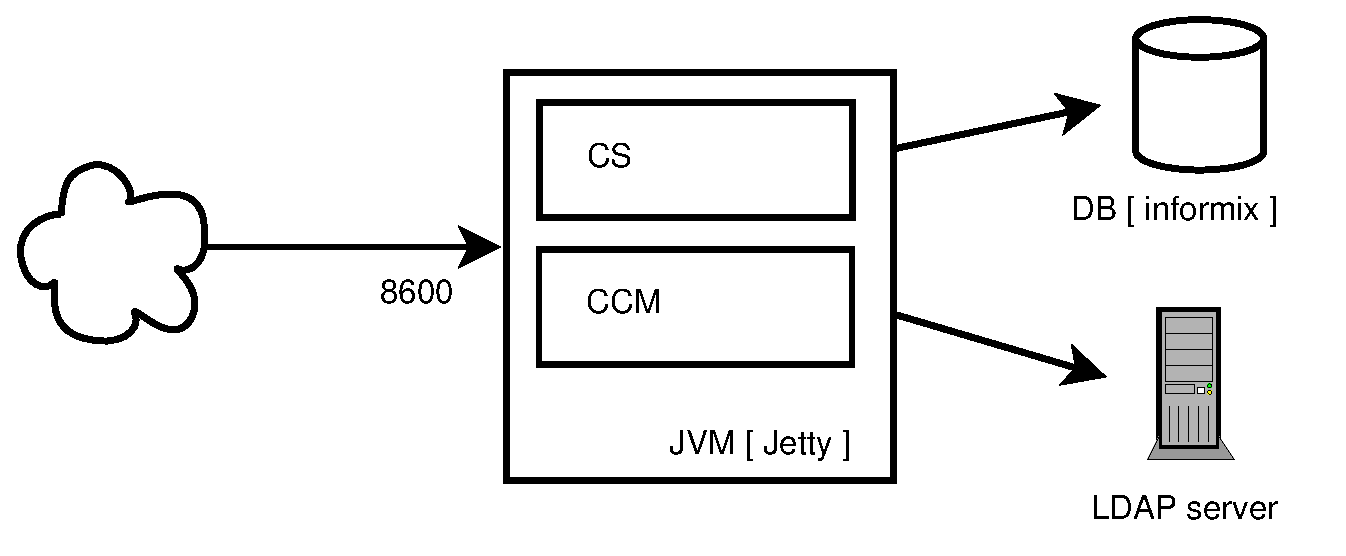
\epsfig{file=cs_diag.eps, width=10cm}
\caption{\cs{} architecture}
\label{fig:cs_diag}
\end{figure}

The LDAP server can either be the server furnished by Telelogic or an external source to plug into enterprise resources.

Oracle and Informix databases are supported by \cm{} -- but the former is limited to Solaris, HP-UX (and AIX for \cm{} 6.3).

\section{Important files}
\label{sec_important_files}

Below is the location for some of the more important \cs{} files:

\begin{description}

\item[\cshome{}/cs\_apps/csctl.sh] The script which starts \cs{} daemons. It should be invoked with the \ccmroot{} user, after the LDAP is connected (i.e. after the \verb!vde.sh! script is invoked if the internal LDAP is used). 

\item[\vdehome{}/vde.sh] The script to start/stop the LDAP server furnished by Telelogic. It should be invoked with the \ccmroot{} user, before the \cs{} daemons are invoked.

\item[\ccmhome{}/etc/license\_data] The file which contains licensing data, as provided by Telelogic.

\item[\ccmhome{}/etc/.router.adr] contains the name of the router host and its IP address.

\item[\ccmhome{}/etc/esd.adr] contains the name of the esd host and its IP address.

\item[\ccmhome{}/etc/ccm\_websrv.adr] contains the name of the webserver host and its IP address.

\item[\webinf{}/wsconfig/] contains most configuration files (e.g. pt.cfg, see \ref{sec:pt.cfg} on page \pageref{sec:pt.cfg}).

\item[\webinf{}/wsconfig/triggers/] contains all triggers defined for the current workflow (see section on triggers, \S \ref{sec:triggers} on page \pageref{sec:triggers}).

\item[\webinf{}/wsconfig/tmpdir/] contains log files (e.g. pt.log).

\item[\webinf{}/wsconfig/templates/pt/include/motd.js] contains the text to be displayed below the login screen. 

\item[\webinf{}/packages/] is the directory containing all packages (installed/uninstalled).

\item[\webinf{}/crprocess/] contains all XML process files.
\end{description}


\section{Setup}

\subsection{Requirements}

\cs{} is far less ressources-consuming than its main competitor Rational ClearQuest. A single server, hosting both backend sessions and database, can handle seamlessly a hundred of activ users and several thousands of records. 

Administration tasks are nevertheless still mandatory, and a full-time administrator -- as for any other software -- is mandatory. For full user satisfaction and efficiency consider hiring one administrator for 100 activ users.

On the client side, the web approach delivers all its flexibility and power; no heavy software setup is necessary. A simple web browser is all that is needed to connect from any location in the world.


\subsection{Patches}

Patches are provided by Telelogic and are freely available on their website\footnote{If you have a valid account..}. All instructions are provided in the README file of each patch and \emph{must be read}. Applying a patch is usually harmless; but the principle of precaution suggests that your database should be backed up. Refer to section \ref{sec:maint_backup} on page \pageref{sec:maint_backup} for this. 

Install instructions vary from one patch to another. \emph{Really always check the readme instructions} provided with the package, since there may be patch-specific hints. In general, patches are reversible: check instructions in the README.

\subsubsection{CCM patches}

The usual way to install a \ccm{} patch is through the ccm\_patch utility. 

\begin{enumerate}
\item Get and install the latest ccm\_patch utility: it can be retrieved with ftp from \verb!ftp.continuus.com/pub/patches/!. Login as anonymous and get \verb!ccm_patch! and \verb!ccm_patch_README!. You should always check that the version of the utility is the latest available. You will also need the \verb!ncompress! utility\footnote{The ncompress utility is NOT installed as a default package in the RedHat E.L. 2.1.}.
\item Shutdown the database:
\begin{verbatim}
$ ccmdb shutdown /path/to/db
\end{verbatim}
\item Read documentation with the \verb!-readme! switch and apply the patch. You must be root to run it, the script changes the user to \ccmroot{} when needed.
\begin{verbatim}
$ ccm_patch -readme patch_6.3 > readme_patch_6.3.txt
$ less readme_patch_6.3.txt
$ su -
# ccm_patch patch_6.3
# exit
\end{verbatim}
\item Unprotect the database:
\begin{verbatim}
$ ccmdb unprotect /path/to/db
\end{verbatim}
\end{enumerate}

\subsubsection{CS patches}

Patches for the \cs{} engine are installed through the Admin web interface (Admin section, CSPackage tab).

\begin{enumerate}
\item Untar the patch file (although it has no .tar extension) and copy it to the \webinf{}/packages directory. 
\begin{verbatim}
$ tar xf patch_cs4.3-030 
$ ls cs4.3-030/
README.txt  VERSION.txt  trapeze  wsconfig
$ cp cs4.3-030/ \webinf{}/packages/
\end{verbatim}
\item Login to \cs{} as Admin, go into the Admin section, CSPackage tab. The patch should appear in the left listbox, among other uninstalled packages. Install it.
\end{enumerate}


\section{The Perl API}

A Perl API is provided by Telelogic and bundled with \cs{}. Almost all operations can be scripted, from administration to reports or submitting. Some of the most useful features of the Perl API can be found below:

\begin{itemize}
\item Records:
\begin{itemize}
\item Get reports, queries.
\item Find records, and get complete attributes set.
\end{itemize}
\item Users:
\begin{itemize}
\item Create, edit and delete users.
\item Add, edit or retrieve users preferences.
\end{itemize}
\item Administration
\begin{itemize}
\item Reload one or all of the configuration files.
\item Set debuging mode to true or false.
\item Get or delete the current log file.
\end{itemize}
\end{itemize}

It is very common to use Perl scripts in lifecycle triggers, either pre-condition for checks or post-condition for actions. The diversity of Perl modules, combined with the flexibility of the language, allow almost any operation or integration.


\section{Scripts}

The Perl API deserves several goals, from server administration to periodic reporting. The scripts provided in the appendix page \pageref{sec:getreport.pl} provide a template that you can safely use and adapt to your environment. POD (in-line) documentation is available, as well as usage through the \verb!-h!switch.

Maintenance scripts are especially useful when used in cron tabs. They allow a delayed check of consistency in the database, update of computed values, batch treatment to export data toward other tools, periodic reporting and statistics, and more\footnote{The scripts are also available online: \href{http://csapi.berlios.de/cs\_admin/}{csapi.berlios.de/cs\_admin/}.}.

One more remark: these scripts have been developed and tested on a Perl 5.6.1 environment, but some (rare) environments won't work (possibly missing modules).

\subsection{Get a report}

The getreport.pl script (see \S \ref{sec:getreport.pl} on page \pageref{sec:getreport.pl}) retrieves attributes for either a query or a set of problem\_number's, provided on the standard input (standard input is intended for piped commands).

\begin{verbatim}
getreport.pl [-h] [-f format ] [-q query] attributes
\end{verbatim}

The list of attributes to be retrieved must be passed on command line, separated by spaces. The ouput can be formatted with the -f switch (using the classic C syntax, cf. man fprintf). 

\begin{verbatim}
$ getreport.pl -f "[%s] %s|%s|%s" -q "(software match 'good*')" 
"problem_number|problem_synopsis|software_platform|software_version" 
[12990] search fails|embedded|2.3
[14851] generated html does not validate|server|2.1
[14928] dead links|server|2.1
\end{verbatim}%$


\subsection{Modify records}

This script (see \S \ref{sec:modifyrecord.pl} on page \pageref{sec:modifyrecord.pl}) allows an user to modify a record on the \cs{} server, according to his rights. A list of problem\_number's can be furnished on command-line, for batch treatments. The synopsis of the script is:

\begin{verbatim}
modifyrecord.pl [-h|help] [-i|identifier identifier] attribute value
\end{verbatim}

It uses an array to store problem\_number's. It either push id furnished on command line or read and push from standard input. For each element of the array, it retrieves an object (getCRData), read (getValue) and set (setValue) the value of the attribute specified on command line. A line is shown with old and new values, along with corresponding problem\_number.

\subsection{Power of CLI}

Command-Line Interface comes handy for mass treatments. The getreport and modifyrecord scripts can be piped to achieve fine-tuned treatments. A classic example could be ``change all records with release 2.1 to release 3.0 in project website''. A way to achieve this request could be: 

\begin{verbatim}
$ getreport.pl -q (release='2.1' and project='website') problem_number
| modifyrecord.pl release '3.0'
\end{verbatim}

\chapter{Maintenance}

\section{Starting and Stopping the server}
\label{section:start_stop_server}

Since \cs{} is built upon several layers, they all have to be started sequentially, with correct user privileges. When su-ing to \ccmroot{} or informix users, the dash option (\verb!su - ccm_root!) should always be used to set correct environment variables.

You could get into troubles if the user starting the daemons is not correct. Right problems happen, and can e.g. forbid the engine to start the sessions. There should be no file with a root owner in the \cshome{} directory (and recursively); you can check it with a quick find:

\begin{verbatim}
$ find ${CS_HOME} -user root
$
\end{verbatim}

A script is probably the best option: it will spare the administrator some time while ensuring the commands are always the same\footnote{Even early in the morning, before the first cup of coffee\ldots}. A script for \cs{} 4.3 is provided in appendix \ref{sec:synergy4.3} on page \pageref{sec:synergy4.3} for your convenience. An alternative version for \cs{} 4.4 is also furnished on the homepage of the project\footnote{\href{http://csapi.berlios.de/cs\_admin/}{csapi.berlios.de/cs\_admin/}}.

As user Informix, start the database (if there is only one database, you can omit the -s flag):
\begin{verbatim}
$ ccmsrv online -y -s /path/to/db
\end{verbatim}

As user \ccmroot{}, start the \ccm{} daemons, the LDAP server (if needed, i.e. if the Telelogic local LDAP server is used) and the \cs{} daemons\footnote{Beware of path issues, vde and csctl need specific entries in the path (see section \ref{sec_important_files} for details).}: 
\begin{verbatim}
$ ccm_start_daemons
$ vde.sh start
$ csctl.sh start
\end{verbatim}

Order does matter. Starting the \cs{} daemons when there is no active LDAP connection may cause a mess in the connections opened by the engine\footnote{And several CLOSE\_WAIT may appear in the output of \texttt{netstat -na}. When there are too many of these (thousands) the server may become unresponsive. The only issue we've found so far is to reset all CLOSE\_WAIT'd sockets through a script and restart all daemons --- or reboot the server.}. When stopping the server, the reverse steps have to be followed. As user \ccmroot{} type:
\begin{verbatim}
$ csctl.sh stop
$ vde.sh stop
$ ccm_stop_daemons
\end{verbatim}

And as user Informix, type (-s flag is optional if there is only one db):
\begin{verbatim}
$ ccmsrv offline -y -s /path/to/db
\end{verbatim}%$


There is an issue here: if a {\tt csctl.sh start} gives {\tt already running\ldots}, and you are sure it is not, you probably did not shutdown correctly the host. 

When stopping the running host, you must always shutdown the CS server, then the LDAP server (if you have one), then the \ccm{} daemons and the Informix DB. This allows all daemons and processes to end gracefully, and to remove any lock file. If you do not follow these steps carefully, and restart the application, it will look for a few locks files, find it and believe it is running.

There are two options here: remove the lock file manually, or use the commands to shutdown the application, which will remove the files for you. After this step, you can start your \ccm{} daemons, csctl.sh and vde.sh scripts. 


\section{Backups}
\label{sec:maint_backup}

\cs{} is probably a vital part of your company's information system, and as such it should be backed up often. \cs{} {\em can} introduce inconsistencies in the database, fire could spread across your datacenter or a black hat could erase half of the records. Ok, \cs{} {\em needs} backups.

This part addresses only the pure \cs{} method of backup and restoration using the ccmdb command set. Other backup methods (such as full system backups) can also be used -- but be warned that the database needs specific backup.

The LDAP server within C/S maintains a local backup schema, executed once every midnight (approx). The backups are stored in: \vdehome{}\verb!/vde/backup/!. Files are in zip format, you can use unzip (UNIX) to extract the files, which should go into \vdehome{}\verb!/vde/data!. Prior to copying files back to the data sub dir, the LDAP server needs to be taken down... 

\subsection{Backup}

Backups need a stop of the \cs{} engine and the database. To ensure that users won't use the database, the LDAP server can also be stopped. As user \ccmroot{}, the following commands stop the application, do the backup and restart all daemons. The backup is a compressed .cpk file.

\begin{verbatim}
$ csctl.sh stop
$ vde.sh stop
$ ccmdb shutdown /path/to/db
$ ccmdb backup /path/to/db -t /path/to/backup
$ ccmdb unprotect /path/to/db
$ vde.sh start
$ csctl.sh start
\end{verbatim}

Carefully look at the output generated by the ccmdb commands: the ccmdb\_backup command looks for inconsistencies before backup by running a ccmdb check. Note that the later can be executed as a stand-alone run, and should be executed daily (but you should have a backup daily anyway).

\subsection{Restore}

To restore a database, get the \verb!.cpk! file. Check that the path to your database is the same that the one used in the originating .cpk file (e.g. if you have more than one host running \cs{}), or every User-Defined query, queryformat or report will be lost.

Basically, the procedure is the same that the one used for backup: shutdown all daemons, unpack and restart all daemons. The ccmsrv has to be online too. As user \ccmroot{}, issue the following commands:

\begin{verbatim}
$ csctl.sh stop
$ vde.sh stop
$ ccm_stop_daemons
$ ccmdb unpack backup.cpk -t /path/to/my_new_db
$ ccm_start_daemons
$ vde.sh start
$ csctl.sh start
\end{verbatim}

After the unpack of the database, you should add it in the admin web interface. Go in 'Admin/Server' tab, Databases section (on left), click on 'Add', enter the full name of the new database (\verb!/path/to/my_new_db! in our example) and fulfill description and label.


\section{Reporting}

A few statistics can be gathered from \cs{}, for a pen-test measure or through a cron job. In the later case, storing values and graphing them in a convenient manner (e.g. with gnuplot) is straightforward.

\begin{description}

\item[ccm\_monitor:] \label{sec:backend_sessions} gives the number of sessions and the path to their database. This should be approximately the ratio of the number of users connected on the number of users per session as defined in the Server tab of the Admin web interface.

\item[ccm\_lmgr\_status:] \label{plain:ccm_lmgr_status} gives licenses usage (who is connected, and what tool is used -- CM Synergy or Change Synergy). It also gives the total number of available licenses. It can be easily parsed with a little bit of awk or Perl magic.

\item[ccmsrv status:] provides information relative to databases.

\end{description}


\section{Defragment the DB}

Apart from an earthquake or alien intrusion in your server, backups will also be used for the Informix database defragmentation. After a long run time (say, a few months of intensive usage) the database becomes fragmented; and there is no tool to defragment it with \ccm{}. 

When the application faces performance issues, it is usually a good idea to plan a maintenance operation, backup the database, delete and unpack it. The full re-insertion of all elements will re-order file fragments and speed up transactions.

Deletion of the current database is done with the {\texttt ccmdb delete} command. Basically, the path to the db is the one you specify when invoking the ccmdb commands; but simply (re)moving the directory is a bad idea. The {\texttt ccmdb delete} not only removes it, but also do other changes in the server internals. This step should be achieved once the backup file has been verified.

Once backups have been made, stop the daemons, delete the database, start the daemons. As user \ccmroot{} commands are:
\begin{verbatim}
$ csctl.sh stop
$ vde.sh stop
$ ccm_stop_daemons
$ ccmdb delete /path/to/db
$ ccm_start_daemons
$ vde.sh start
$ csctl.sh start
\end{verbatim}

You can then unpack your database at the same location: 

\begin{verbatim}
$ ccmdb unpack /path/to/backup.cpk -t /path/to/db
\end{verbatim}

Check that the database is recognized in the Admin web interface, section Server (it should be enabled) and check backend sessions are running (see � \ref{sec:backend_sessions} on page \pageref{sec:backend_sessions}).


\section{Expand the DB space}

The Informix database uses four dbspaces, specified on installation: rootdbs, temp, log, ccm. If the workload of the server is surprisingly increasing more than expected, these dbspaces may fulfill quickly. In this section, we will study how DB space can be increased.

You should have a look at some technical pages from the Telelogic support web site\footnote{https://support.telelogic.com/en/synergy/kb/}: TB206 -- Increasing the Logical Logs in Informix On-Line 7.x and 9.x (UNIX and NT) and TB217 -- Expanding An Informix On-Line 7.x or 9.x Database Server (UNIX). Also refer to the \ccm{} Synergy Administration Guide for \unix{}.

A dbspace is divided into \emph{logical logs}, which are storage areas for transactions (i.e. actions made on the server) before they are processed. When processing (checkpoint) occurs\footnote{Checkpoints are defined by default to run every 5 minutes.}, all data are cleaned from the logical logs for future use, e.g. like in a fifo.

So, the amount of memory used in dbspaces should remain approximately identical, excepted when the real-time workload increases significantly. You should monitor dbspace usage; when occupation exceeds 70\%, consider adding some more chunks of free space.

\paragraph{The ccm logspace} holds all informations about objects created by users. Especially, if you use a lot of strings in the creation of, say a CR, this dbspace will fulfill quickly\footnote{When installing \cs{}, the ccm dbspace is approximately twice as big as others, making it the biggest dbspace available amongst the four created.} --- attributes are stored elsewhere, in the st\_root directory.

Some statistics about dbspace level of usage can be obtained by issuing the following command: 

\begin{verbatim}
$ ccmsrv status -d

*** database server kadath ***

server number:          1
state:                  On-Line

[..SNIP..]

--- dbspace rootdbs ---
total free space:       151608 Kbytes
chunk files: 
/chunkfiles/kadath_root.dbs 171504 Kbytes total, 151608 Kbytes free

--- dbspace temp ---
total free space:       171398 Kbytes
chunk files: 
/chunkfiles/kadath_temp.dbs 171504 Kbytes total, 171398 Kbytes free

--- dbspace log ---
total free space:       6038 Kbytes
chunk files: 
/chunkfiles/kadath_log.dbs 41984 Kbytes total, 6038 Kbytes free

--- dbspace ccm ---
total free space:       48724 Kbytes
chunk files:
/chunkfiles/kadath_ccm.dbs 307200 Kbytes total, 12 Kbytes free
/chunkfiles/kadath_ccm_2.dbs 200000 Kbytes total, 736 Kbytes free
\end{verbatim}

To do the expansion, you have to add a chunk file to the selected dbspace. To add a new chunk file of size \verb!new_size! in the ccm dbspace, use the following command: 
\begin{verbatim}
$ ccmsrv expand -size new_size -path /path/to/chunkfiles/ -y 
 -dbspace ccm
\end{verbatim}%$

After the command exits, a new chunkfiles has been created, and a \verb!ccmsrv status -d! shows a new line.

\begin{verbatim}
--- dbspace ccm ---
total free space:       48724 Kbytes
chunk files:
/chunkfiles/kadath_ccm.dbs 307200 Kbytes total, 12 Kbytes free
/chunkfiles/kadath_ccm_2.dbs 200000 Kbytes total, 736 Kbytes free
/chunkfiles/kadath_ccm_3.dbs 200000 Kbytes total, 199374 Kbytes free
\end{verbatim}


\chapter{Customizing \cs{}}

\cs{} can be highly fine-tuned and customized to feet into the company's traditions. 

First, the workflow for record management used in the company can be reproduced, with all states, transitions, attributes and rights. When implementation becomes tricky using the default features, triggers can provide a way to external resources or execute some complex operation, e.g. to grant rights.


\section{Triggers}
\label{sec:triggers}

Triggers can be written in Perl or shell. They are scripts executed on given events: transition, attribute modification, etc. and are specified in the lifecycle. Three types of triggers can be set in a workflow: 

% XXX add ptcli.cfg pre-condition triggers 

\begin{description}
\item[pre-condition triggers] are executed {\em before} a transition, and can eventually forbid it by returning 1 (one). A zero (0) return code indicates that the transition is allowed. Additionally, a {\tt die} command prints a message on the bottom of the generated page, which is useful to explain the reason of refusal.
\item[post-condition triggers] are executed {\em after} a transition is passed, and thus cannot prevent it to happen. They can be used to compute the value of an attribute, send an email to e.g. the assigned engineer, or update some third-party tool.
\item[attribute modification triggers] are fired when a specified attribute is modified, either while in a state or on transition. Modification attributes are set in the lifecycle editing facilities, Edit CRProcess, Attributes.
\end{description}

On attribute modification, only post-condition triggers can be defined. This is a bad thing, since we cannot check the content of the attribute and prevent the modification if something is wrong. But, at last, it allows operations on the new value.

If a check on an attribute value is mandatory, e.g. for conformance to a given format, it may still be accomplished through a modification trigger. Although it is somewhat complex, the following method can be used:

\begin{enumerate}
\item read the transition log;
\item parse and extract the last value of the attribute checked before modification occured;
\item modify the attribute and set it back to the original value.
\end{enumerate}

% XXX add modification trigger script

Beware of loops: if you change the value of the attribute, the modification trigger will be re-fired, and re-executed. Thus a flag must be set and checked before any action.


\section{Configuration files}
\label{sec:conf_files}

Configuration files are divided into sections, containing lines of the form given thereafter. One section can have several lines attached; one line can have several parameters. The whole \verb!CFG_SECTION! must be on one line; it can contain several \verb!CFG_PARAM!; it seems that the order of \verb!CFG_PARAM! does not matter.

\begin{verbatim}
[CFG_SECTION]
  [CFG_PARAM]param1|param2|param3[/CFG_PARAM]
[/CFG_SECTION]
\end{verbatim}

There are several configuration files in the wsconfig directory\footnote{the wsconfig directory is located in \webinf{}\-/wsconfig.}. Some of them are directly used by \cs{}, others are installed along with packages. 

We will first address two main configuration files, \verb!pt.cfg! and \verb!pt_listbox.cfg!, then study how other configuration files from the \webinf{}\-\verb!/wsconfig! are built.

\subsection{The pt.cfg configuration file}
\label{sec:pt.cfg}

It is the main configuration file for \cs{}. As stated in the preamble of the file, 

\begin{quote}
``This is the main Change Synergy configuration file. Changes to this file should be limited to the System Variables Section. Additional changes should be done in a custom configuration file and referenced here using the CFG\_MERGE setting.''
\end{quote}

This file defines among others session, databases and hosts parameters, LDAP settings, the behavior of stand-alone windows (e.g. when you ask for a report), HTTP parameters, date formats, entities encoding, tasks and objects options.

\label{plain:cfg_merge}
The CFG\_MERGE section lists configuration files to be parsed in the current directory (wsconfig) after the pt.cfg file. When the administrator installs a package in the web administration interface, the name of the cfg file of the package is appended to the end of this section.

\begin{verbatim}
[CCM_SYSTEM]
  [CFG_MERGE]
    sub_attachment.cfg|sub_duplicates.cfg|my_report.cfg
  [/CFG_MERGE]
[/CCM_SYSTEM]
\end{verbatim}

The parsing order is the one specified in the pt.cfg file. Thus any declaration occurring more than once in the cfg files may be overwritten by a new occurrence, depending on the configuration of the package. As a result, \emph{the order of installation of packages does matter}.

If \cs{} is used for purposes other than change requests, it may be interesting to change the name of items from ``Change Request'' to, say ``Document Request''. This can be achieved by changing elements of the \texttt{Textual Replacement Variables} section: \verb!Problem_Identifier!, \verb!Problem_Identifier_Plural!, \verb!Problem_Identifier_Abbr!.

\begin{verbatim}
[CCM_ATTRIBUTE]
  [NAME]Problem_Identifier[/NAME
  [ALIAS]Document Request[/ALIAS] # instead of Change Request
  [TYPE]CCM_STRING[/TYPE]
[/CCM_ATTRIBUTE]
\end{verbatim}

\subsection{The pt\_listbox.cfg configuration file}

pt\_listbox.cfg contains the definition of all listboxes, as shown in the Listbox section of the Admin web interface.

Since there may be dependent listboxes, this file can quickly become confusing and should as far as possible not be edited by hand. One exception is when \cs{} itself falls and messes items; in which case you will have to investigate yourself. But, in any case, remember to often backup your wsconfig directory.

\section{Template}

An important part of configuration files present in the \verb!wsconfig! directory address package-specific customizations. The items studied here can be needed e.g. to customize listboxes (e.g. hide the SimpleProcessQuery in the CustomQuery), or restrict access to specific parts of the web interface.

As stated in section \ref{sec:server_architecture}, the \jetty{} engine uses templates to build the HTML pages. These templates are located in the \webinf{}/wsconfig/templates/pt directory, and can be customized. The main difficulty is the understanding of the template itself: \cs{} defines \wslet{}, which are on-the-fly replacements by e.g. database data. 

It is quite straightforward to remove an item. Templates can easily be modified to hide or show some parts of the interface, such as one of the top buttons as explained in \S \ref{sec:custUI}. Customization for a particular \csrole{}\footnote{Remember that different \csrole{} can (and usually) have different web interfaces.} has two steps:

\begin{description}
\item[Create a link to the new template] through a configuration file indicating the path of the template to be used. Report definitions use it to format the report display (see \S \ref{sec:ccm_problem} on page \pageref{sec:ccm_problem}), but it can also be used to completely redefine the main UI with the \verb!CCM_TEMPLATE! declaration -- see below.
\item[Create the template] by modifying and saving as one of the files present in the \verb!wsconfig! directory. 
\end{description}

To hide or show UI parts, the main configuration item is \verb!CCM_TEMPLATE!.

\begin{verbatim}
[CCM_TEMPLATE]
  [NAME][/NAME]
  [ATTRS][/ATTRS]
  [FILE][/FILE]
  [ONLOAD_ACTION][/ONLOAD_ACTION]
  [CSRole_a][/CSRole_a]
  [CSRole_b][/CSRole_b]
[/CCM_TEMPLATE]
\end{verbatim}

\begin{itemize}
\item \verb!NAME! is the name of the \verb!CCM_TEMPLATE! declaration.
\item \verb!ATTRS! is a list of attributes, separated by pipes. Depending on the configuration file, pipe-separated items may be only the name of the attribute (e.g. in crprocess\_xx.xml) or a 3-uple: \{attribute name, $-1$, false\}:
\item \verb!ONLOAD_ACTION! contains the name of the corresponding action.
\item \verb!FILE! is the path of the file to be loaded (if no \csrole{} has been specified on the line). 
\item \verb!ROLE NAME! specifies which file to load for this particular \csrole{}.
\end{itemize}

As shown below, the admin\_framework.cfg contains one \verb!CCM_TEMPLATE! definition including two \csroles{}: Admin and ReportBuilder. The template loaded for an Admin \csrole{} would in this case be admin\_framework/buttonbar\_panel\_admin.html, and for a ReportBuilder \csrole{} admin\_framework/buttonbar\_panel\_reportbuilder.html. Paths are relative to the \webinf{}/wsconfig/templates/pt/forms/ directory.

\begin{verbatim}
[CCM_TEMPLATE]
  [NAME]ButtonBar[/NAME]
  [ONLOAD_ACTION]main_buttonbar_form[/ONLOAD_ACTION]
  [Admin]admin_framework/buttonbar_panel_admin.html[/Admin]
  [ReportBuilder]admin_framework/buttonbar_panel_reportbuilder.html[/ReportBuilder]
[/CCM_TEMPLATE]
\end{verbatim}

As often, an example is far better than 1000 words: we will study in section \ref{sec:custUI} how a configuration file can add or replace some elements of the user interface, using templates.


\subsection{CCM\_LIST}

For reports, the \verb!CCM_LIST! section takes care of listboxes display. There are three listboxes available (Query, Format, Report), which can be declined\footnote{Users can have different lists of reports depending on the lifecycle they select in the top-left box of the Report section.} in as many versions as defined lifecycles, plus one for the 'All Lifecycles' item. \verb!CCM_LIST! lines have the following parameters:

\begin{verbatim}
[CCM_LIST]
  [NAME][/NAME]
  [SECTION][/SECTION]
  [VALUES][/VALUES]
  [APPEND][/APPEND]
[/CCM_LIST]
\end{verbatim}

\begin{description}
\item \verb!NAME! can address a specific workflow by just adding its short name at the end of the selected listbox name; say we have defined two workflows, one for Document Requests (short: doc) and another for Typography Fixes (short: typo). The listboxes could have the following names (we just list items for the Document Requests and All workflows items):

\label{plain:crquerycustom}
\begin{itemize}
\item For All Workflows:
\begin{itemize}
\item CRQueryPreDefined: Pre-Defined Queries listbox,
\item CRQueryUserDefined: User-Defined Queries listbox,
\item CRQueryCustom: Custom Queries listbox,
\item CRQueryShared: Shared Queries listbox,

\item CRQueryReportPreDefined: Pre-Defined Formats listbox,
\item CRQueryReportUserDefined: User-Defined Formats listbox,
\item CRQueryReportCustom: Custom Formats listbox,
\item CRQueryReportShared: Shared Formats listbox,

\item CRReportPreDefined: Pre-Defined Reports listbox,
\item CRReportUserDefined: User-Defined Reports listbox,
\item CRReportCustom Custom: Reports listbox,
\item CRReportShared: Shared Reports listbox.
\end{itemize}

\item For Document Requests:
\begin{itemize}
\item CRQueryPredefined\_doc Pre-Defined Queries listbox,
\item CRQueryUserdefined\_doc User-Defined Queries listbox,
\item CRQueryCustom\_doc Custom Queries listbox,
\item CRQueryShared\_doc Shared Queries listbox,

\item CRQueryReportPreDefined\_doc Pre-Defined Formats listbox, 
\item CRQueryReportUserDefined\_doc User-Defined Formats listbox, 
\item CRQueryReportCustom\_doc Custom Formats listbox, 
\item CRQueryReportShared\_doc Shared Formats listbox, 

\item CRReportPreDefined\_doc Pre-Defined Reports listbox,
\item CRReportUserDefined\_doc User-Defined Reports listbox,
\item CRReportCustom\_doc Custom Reports listbox,
\item CRReportShared\_doc Shared Reports listbox.
\end{itemize}
\end{itemize}

\item \verb!SECTION! is the type of item to add; it can be one of \verb!CCM_REPORT! (for Reports and Formats) or \verb!CCM_QUERY! (for Queries only).

\item \verb!VALUES! is a pipe-separated list of either report names or query names to be displayed in the selected listbox, as specified in other lines. The names must be \emph{exactly the same} than those defined in the \verb!NAME! section of the declaration. Beware of spaces and case.

\item \verb!APPEND! is a boolean value. If it is set to true (normal behavior) the declaration will be appended to the existing list of reports to show. It set to false, any preceding value will be replaced by the current one. If other reports are specified later on, with a true \verb!APPEND! option, they will be appended to the current list. This allows to easily erase a whole listbox and redefine its content.
\end{description}


\subsection{CCM\_QUERY}

The \verb!CCM_QUERY! lines define the query strings to be executed. One query string can be used by several \verb!CCM_LIST! (e.g. in our preceding example, the CRQueryPreDefined, the CRQueryPreDefined\_doc and CRQueryPreDefined\_typo listboxes could point to the same \verb!CCM_QUERY!). 

\begin{verbatim}
[CCM_QUERY]
  [QRY_STRING][/QRY_STRING]
  [QRY_TEMPLATE]CCM_QUERY[/QRY_TEMPLATE]
  [DESCRIPTION]All Documents[/DESCRIPTION]
  [DATE_LAST_RUN][/DATE_LAST_RUN]
[/CCM_LIST]
\end{verbatim}

\begin{description}
\item \verb!QRY_STRING! is the full query string, as it would be written in the web interface, e.g. \verb!(cvtype='problem')! \verb!and! \verb!(problem_synopsis match '*todo*')!.

\item \verb!QRY_TEMPLATE! is most of the time empty. Only some auto-generated lines (e.g. in the cr\_process.xml workflow definition) have this option filled.

\item \verb!DESCRIPTION! and \verb!DATE_LAST_RUN! are self-descriptive. The description is used when displaying the query, and the date of last run is used by \cs{} to rerun reports in the Report Folder --- Recent Reports.
\end{description}


\subsection{CCM\_REPORT}
\label{sec:ccm_report}

\begin{verbatim}
[CCM_REPORT]
  [NAME][/NAME]
  [RPT_TEMPLATE][/RPT_TEMPLATE]
  [QUERY][/QUERY]
  [PROBLEM_DEF][/PROBLEM_DEF]
  [EXPORT_FORMAT][/EXPORT_FORMAT]
  [MAX_QUERY][/MAX_QUERY]
  [MAX_STRING][/MAX_STRING]
  [INCREMENTAL][/INCREMENTAL]
  [INCREMENT_SIZE][/INCREMENT_SIZE]
  [DESCRIPTION][/DESCRIPTION]
[/CCM_REPORT]
\end{verbatim}

The \verb!CCM_REPORT! lines define the reports (CRQueryReport or CRReport).

\begin{description}
\item \verb!NAME! must be identical (spaces, case) to the name specified in the \verb!CCM_LIST! element.

\item \verb!RPT_TEMPLATE! is the name of a \verb!CCM_TEMPLATE! definition. The name must be exactly the same. Beware of spaces and case.

\item \verb!QUERY! is the \verb!CCM_QUERY! item to be used with this report. If the \verb!CCM_REPORT! is to be applied to a CRQueryReport (which does not need a query string) the parameter is discarded. The name of the Query must be exactly the same. Beware of spaces and case.

\item \verb!PROBLEM_DEF! is a reference to a \verb!CCM_PROBLEM! line to define the format of the reported records (attributes used, grouping, etc. see \S \ref{sec:ccm_problem} below). Beware of spaces and case.

\item \verb!EXPORT_FORMAT! describes the export format; it is one of \verb!HTML!, \verb!CSV!, \verb!XLS!, \verb!RTF!, \verb!XML!.

\item \verb!MAX_QUERY! is the maximum number of records to be included in the report. The reports fails if this limit is reached.

\item \verb!MAX_STRING! is the maximum string length of any attribute reported. If this limit is reached, the attribute value is truncated.

\item \verb!INCREMENTAL! is a boolean value to indicate if the report is displayed incrementally (i.e. on several pages, with next and previous links) or nor (all records on one page).

\item \verb!INCREMENT_SIZE! specifies the number of records per page when the incremental mode is selected.

\item \verb!DESCRIPTION! is a free description of the \verb!CCM_REPORT!.
\end{description}

\subsection{CCM\_PROBLEM}
\label{sec:ccm_problem}

The \verb!CCM_PROBLEM! line defines the way attributes will be displayed in the report. It is somewhat problematic for customization, since it make calls to templates created at report installatino time. 

When customizing, the csreports packages won't install if this line because of this line. It must not be included in the customized file, but instead used directly with the original \verb!CCM_PROBLEM! installed with the original report.

\begin{verbatim}
[CCM_PROBLEM]
  [NAME][/NAME]
  [ATTRS][/ATTRS]
  [SORT_ORDER][/SORT_ORDER]
  [MAIN_TEMPLATE][/MAIN_TEMPLATE]
  [HDR_TEMPLATE][/HDR_TEMPLATE]
  [ATTR_TEMPLATE][/ATTR_TEMPLATE]
  [IMG_TEMPLATE][/IMG_TEMPLATE]
  [GROUP_BY][/GROUP_BY]
  [GROUP_TEMPLATE][/GROUP_TEMPLATE]
  [FTR_TEMPLATE][/FTR_TEMPLATE]
  [LABEL_TEMPLATE][/LABEL_TEMPLATE]
  [AUTO_LABEL_TEMPLATE][/AUTO_LABEL_TEMPLATE]
  [AUTO_ATTR_TEMPLATE][/AUTO_ATTR_TEMPLATE]
  [SPAN_ATTR_TEMPLATE][/SPAN_ATTR_TEMPLATE]
  [CUSTOM_WSLET][/CUSTOM_WSLET]
  [XML_CONTENT][/XML_CONTENT]
[/CCM_PROBLEM]
\end{verbatim}

\begin{description}
\item \verb!NAME! is the name of the current \verb!CCM_PROBLEM!. It must be exactly the same than the one used in the \verb!PROBLEM_DEF! reference in \verb!CCM_REPORT!.

\item \verb!ATTRS! is the list of attributes to be displayed for each returned record, separated by pipes. Each item contains three fields separated by colons:
\begin{itemize}
\item the name of the attribute, 
\item its position in the dialog ($-1$ means hidden) and 
\item the \verb!SPAN! boolean (true if the attribute is spanned all along the line, or false if 2-cols paging is used).
\end{itemize}

In the following example, three attributes are displayed the way shown on Figure \ref{fig:ccm_problem_attrs}.
\begin{verbatim}
problem_number:0:false|crstatus:1:false|problem_synopsis:2:true
\end{verbatim}

\begin{center}
\begin{tabular}{|c|c|}
\hline
problem\_number & crstatus \\
\hline
\multicolumn{2}{|c|}{problem\_synopsis} \\
\hline
\end{tabular}
\label{fig:ccm_problem_attrs}
\end{center}

\item \verb!SORT_ORDER! specifies the sort key(s); it is a pipe-separated list of 3-uples, namely:

\begin{itemize}
\item the name of the attribute chosen as sort key, 
\item its type (Integer: int, Integer Back: intb, String: string, etc.). All types are defined in the reports section of the web interface, tab Sorting.
\item a letter defining the sort order: A (ascending) or D (descending).
\end{itemize}

\item \verb!MAIN_TEMPLATE! is the path to the main template.

\item \verb!HDR_TEMPLATE! is the path to the template file to be used for display of header, relative to the WEB-INF/wsconfig directory.

\item \verb!ATTR_TEMPLATE! is the path to the template used for each attribute display, relative to the WEB-INF/wsconfig directory.

\item \verb!IMG_TEMPLATE! is the path to the template used for pictures (charts) display, relative to the WEB-INF/wsconfig directory.

\item \verb!GROUP_BY! is the name of the attribute used to set grouping.

\item \verb!GROUP_TEMPLATE! is the path to the template used for grouping, relative to the WEB-INF/wsconfig directory.

\item \verb!FTR_TEMPLATE! is the path to the template used for the footer display, relative to the WEB-INF/wsconfig directory.

\item \verb!LABEL_TEMPLATE! is the path to the template used for labels. Almost never used, relative to the WEB-INF/wsconfig directory.

\item \verb!AUTO_LABEL_TEMPLATE! is the path to the template used for auto-labels. Almost never used, relative to the WEB-INF/wsconfig directory.

\item \verb!AUTO_ATTR_TEMPLATE! is the path to the template used for auto-attributes. Almost never used, relative to the WEB-INF/wsconfig directory.

\item \verb!SPAN_ATTR_TEMPLATE! is the path to the template used for spanned attributes, relative to the WEB-INF/wsconfig directory.

\item \verb!CUSTOM_WSLET! may be used to specify a class file (e.g. CSChartOpenVsClosedTrend, which is a class file located in WEB-INF/classes/com/continuus/webpt/servlet/CSChartOpenVsClosedTrend.class). Almost never used.

\item \verb!XML_CONTENT! is never used in the basic reports furnished.

\end{description}


\section{Packages}
\label{sec:packages}

A package is a set of consistent configuration files, templates and customization items grouped together. It proposes a convenient way to activate/deactivate changes distributed over several files.

Packages are located in \webinf{}/packages/*. The name of the directory is the same than the name of the package when it appears in the admin web interface. Every package contains two files that will help \cs{} to identify the package to install: 
\begin{description}
\item[README.txt] contains a description of the package, instructions for install/uninstall and eventually some recommendations for next developer.
\item[VERSION.txt] contains three lines: the version of \cs{} and the degree of service pack (e.g. 4.3\_sp1), an indication of the application (i.e. \verb!CS!) and the type of package (one of \sc{csreport}, \sc{crprocess}, \sc{customization}, \sc{patch}).
\end{description}

Every file (or directory) from the package will be copied on install in the \webinf{}/ directory, excepted README.txt, VERSION.txt and auto-generated elements. As an example, configuration files must be copied into the \webinf{}/wsconfig directory to be taken into account. That's why most of the packages contain a wsconfig subdir.

\cs{}, upon install of package, also edits the pt.cfg file to add the name of the new configuration file to the CFG\_MERGE section (see in section \ref{plain:cfg_merge} on page \pageref{plain:cfg_merge} for more information about the CFG\_MERGE section).

For the basic\_summary csreport package, one of the default report, we have the arborescence listed in figure \ref{list:basic_summary}. If it has already been installed, a backup directory may have been created automatically, with the date of install (e.g. backup\_16\_05\_2005\_10\_35\_39). The uninstall directory, as well, is automatically created upon install.

In this example, install of the package will copy:
\begin{itemize}
\item report definition file basic\_summary.xml in \webinf{}/cs\_reports,
\item configuration file basic\_summary.cfg in \webinf{}/wsconfig,
\item template files main\_attr\_basic\_summary.txt, main\_hdr\_basic\_summary.txt, main\_rpt\_basic\_summary.txt in \webinf{}/wsconfig/templates/pt/reports/basic\_summary/.
\end{itemize}

\begin{verbatim}
basic_summary/
|-- README.txt
|-- VERSION.txt
|-- cs_reports
|   `-- basic_summary.xml
`-- wsconfig
    |-- basic_summary.cfg
    `-- templates
        `-- pt
            `-- reports
                `-- basic_summary
                    |-- main_attr_basic_summary.txt
                    |-- main_hdr_basic_summary.txt
                    `-- main_rpt_basic_summary.txt
\end{verbatim}
\label{list:basic_summary}

Order of install for packages does matter, as stated in section \ref{plain:cfg_merge}. 

\section{Real-Life examples}

\subsection{The custUI package}
\label{sec:custUI}

In this section, we will apply some of the previously seen aspects of \cs{} customization. We will use a template and a configuration file put together in a package for convenient install/uninstall.

\paragraph{Statement of work}

We want to disable the SimpleProcess query in the CustomQuery section of the web interface, since it does not work. We also want to hide the 'Home' button from the top panel.

\paragraph{Build the package}

To build a package, you first have to create the arborescence of files, and populate it with the templates, configuration files and any file that you wish to install with. In \webinf{}/packages, create a new directory with the name you want to give to your package. Populate it with the following files:

\begin{description}

\item[myPackage/README.txt] contains a description of the package (free form).
\begin{verbatim}
My Own Customization Package

This package demonstrates the building of a 
customization package for Change Synergy. The 
first section removes the SimpleProcessQuery
entry from the Custom Queries listbox, the 
second hides the ``Home'' button from the top 
panel.
\end{verbatim}

\item[myPackage/VERSION.txt] contains three lines: the version of \cs{} it applies to including service pack (e.g. 4.3\_sp3), the \verb!CS! keyword and the type of package (see \S \ref{sec:packages} on page \pageref{sec:packages} for more information on this file).
\begin{verbatim}
4.3_sp1
CS
CUSTOMIZATION
\end{verbatim}

\item[myPackage/wsconfig/myPackage.cfg] will be appended, when installed, to the list of merges in the pt.cfg. It redefines the entries to be shown for the Query Custom listbox (see \S \ref{plain:crquerycustom} on page \pageref{plain:crquerycustom}). Note that the whole \verb!CCM_LIST! must be entered as one line.
\begin{verbatim}
# removes the SimpleProcessQuery entry by
# forcing only the Custom CR and
# the By CR Id entries.
[CCM_LIST]
  [NAME]CRQueryCustom[/NAME]
  [SECTION]CCM_QUERY[/SECTION]
  [VALUES]Custom CR|By CR ID[/VALUES]
  [APPEND]false[/APPEND]
[/CCM_LIST]
\end{verbatim}

\item[myPackage/wsconfig/templates/pt/forms]

\end{description}

\subsection{Adding a \ccmrole{}}
\label{sec:add_ccmrole}

We want to add ReportBuilder \ccmrole{} and \csrole{}. It would allow administrators to add reporting capabilities to specific users through the Web Interface easily. Selected users would then connect with the ReportBuilder role, without needs for any other right.

To create the \ccmrole{}, we have to add it for at last one user in the \cm{} engine. Once created it will remain for future use and will only need to be activated in the User tab of the Admin web interface.
\begin{verbatim}
$ ccm start -d /path/to/db
Starting CM Synergy...
$ ccm set role ccm_admin
$ ccm users
\end{verbatim}

The list of users defined in the \ccm{} engine appears in a vi editor; each line has the current login, with a list of \ccmroles{} separated with spaces. Edit the list and affect to at last one user the reportbuilder \ccmrole{}. Save and Quit. As soon as the \ccmrole{} is declared, it shows in the User Admin tab from the web interface and can be easily affected to users.

\begin{verbatim}
user ccm_root = developer assigner build_mgr ccm_admin 
component_developer concluder dcm_mgr group_mgr pt_admin
tester type_develoepr verifier writer;
user dupond = developer reportbuilder;
user dupont = developer;
\end{verbatim}%$

Stop the \ccm{} session (\verb!ccm stop!), login as Administrator to the web interface, go in the Lifecycle editor and add for the reportbuilder \ccmrole{} a new \csrole{} --- e.g. ReportBuilder. This will allow users without any other \csrole{} to connect only with ReportBuilder. Install the new process package and the ReportBuilder \csrole{} appears in the login page.

Note that users with a ReportBuilder role can crash others sessions, if reports used in your defintion files (customization of listboxes) are removed\footnote{This warning only applies if you have modified the contents of query or reports listboxes, as e.g. described in section \ref{sec:custUI}.}.

\appendix

\chapter{getreport.pl}
\label{sec:getreport.pl}

\begin{verbatim}
#! /usr/bin/perl -w -I/path/to/lib
# replace with your lib path

use strict;
use Getopt::Long;
use ChangeSynergy::csapi;
use Time::gmtime;

# Usage: get_report.pl [-f format] query attributes
# This script is gpl'ed. See www.fsf.org.

my $usage = <<EOU;
usage: $0 [-h] [-f format ] [-q query] attributes

$0 displays a text report with specified attributes;

The records to retrieve are either specified on stdin
or directly specified with a query string. 

If a format string is provided (classic printf C 
format) attributes will follow String format.

$0 -f "[%s] %s|%s|%s" -q "(software match 'good*')" 
"problem_number|problem_synopsis|software_platfo
rm|software_version" 
[12990] search fails|embedded|2.3
[14851] generated html does not validate|server|2.1
[14928] dead links|server|2.1

EOU
die $usage if ($#ARGV == -1);

Getopt::Long::Configure("bundling");

# Set accordingly to your installation
my $SERV_IP = "172.16.152.128";
my $SERV_DB = "/db/ccmdb/test_db";
my $USER_LOGIN = "user";
my $USER_PASSWD = "password";
my $USER_ROLE = "User";

# Variables declaration
my ($user, $results,
    $queryargs, $querystring, 
    $opt_query, $opt_help, 
    $opt_format,
    $identifier, @identifiers);

# Define available options
my $options = GetOptions( 'q|query=s' => \$opt_query,
  'h|help' => \$opt_help, 'f|format:s' => \$opt_format);

die $usage if (defined($opt_help));

# If no query is furnished, build a query to retrieve 
# needed attributes from problem_number given as std 
# input.
if (defined($opt_query)) { $querystring = $opt_query; }
else {
  while (<STDIN>) {
    chomp;
    push @identifiers, $_;
  }
  $identifier = pop @identifiers;
  $querystring = qq/(problem_number='$identifier')/;
  foreach $identifier (@identifiers) {
    $querystring = $querystring . qq/or(problem_number='$identifier')/;
  }
}
    
eval
{
  $queryargs = join "|", @ARGV;

  my $csapi = new ChangeSynergy::csapi();
  $csapi->setUpConnection("http", $SERV_IP, 8600);
  $user = $csapi->Login($USER_LOGIN, $USER_PASSWD, 
                        $USER_ROLE, $SERV_DB);
  
  # Get query data
  $results = $csapi->QueryData($user, "Basic Summary", 
     $querystring, undef, undef, undef, $queryargs);
};

if ($@)
{
  #print $@;
  print "No match. Dying. \n";
  exit 64;
}  

# Loop through the results to display formatted attributes
for (my $i = 0 ; $i < $results->getDataSize() ; $i++) {
  my $report_data = $results->getDataObject($i);
  my @attribute_data;
  my $finalattr;


  for (my $j = 0 ; $j < $report_data->getDataSize() ; $j++) {
    # converts universal time since epoch to modern styles.
    if ($report_data->getDataObject($j)->getType() eq "CCM_DATE") {
      my $gm = gmtime($report_data->getDataObject($j)->getValue());
      $attribute_data[$j] = sprintf "%2.2d%2.2d%2.2d", 
          $gm->year-100, $gm->mon+1, $gm->mday+1;
    } else {
      $attribute_data[$j] = $report_data->getDataObject($j)->getValue();
    }
  }
  if (defined($opt_format)) {
    $finalattr = sprintf $opt_format, @attribute_data;
  } else {
    $finalattr = join "|", @attribute_data;
  }
  print "$finalattr \n";
}

__END__

=pod

=head1 Name

B<getreport.pl> -- Displays specified fields from 
a selection of problem reports.

=head1 Synopsis

Usage: B<getreport.pl> [-h] [-f format ] [-q query] attributes

=head1 Description

$0 displays a text report with specified attributes;

The records to retrieve are either read on stdin
or directly specified with a query string. 

If a format string is provided (classic printf C 
format) attributes will follow String format.

$0 -f "[%s] %s|%s|%s" -q "(software match 'good*')" 
"problem_number|problem_synopsis|software_platform|software_version" 
[12990] search fails|embedded|2.3
[14851] generated html does not validate|server|2.1
[14928] dead links|server|2.1

=cut
\end{verbatim}

\chapter{modifyrecord.pl}
\label{sec:modifyrecord.pl}

\begin{verbatim}
#! /usr/bin/perl -w -I/path/to/lib
# replace with your lib path 
require 5.002;

use strict;
use Socket;
use Carp;
use FileHandle;
use Getopt::Long;
use ChangeSynergy::csapi;

# Usage: modifyrecord.pl [-h|help] [-i|identifie identifier] attribute value
# This script is gpl'ed. See www.fsf.org.

my $usage = <<EOU;
usage: $0 [-h|help] [-i|identifier identifier] attribute value

$0 allows a Change Synergy administrator to set attributes 
for problem_number furnished either on command line (with
the -i switch) or on stdin.

\$ $0 -i 567 problem_synopsis "User should be able to change theme."

EOU
die $usage if ($#ARGV == -1);

Getopt::Long::Configure("bundling");

# Set accordingly to your installation
my $SERV_IP = "172.16.152.128";
my $SERV_DB = "/db/ccmdb/test_db";
my $USER_LOGIN = "user";
my $USER_PASSWD = "password";
my $USER_ROLE = "User";

# variable declaration
my ($record, $identifier, $queryargs, $user, 
    $opt_help, $opt_id);

my (@identifiers, $attribute,
    $old_value, $new_value);

# Define available options
my $options = GetOptions( 'i|identifier=i' => \$opt_id,
  'h|help' => \$opt_help);

# Display usage if help is needed.
die $usage if (defined($opt_help));

# If no id is furnished on command line, get from 
# stdin, one id per line.
if (!defined($opt_id)) {
    while (<STDIN>) {
	chomp;
	push @identifiers, $_;
    }
} else { push @identifiers, $opt_id; }

# Get parameters.
$attribute = shift;
$new_value = shift;

my $csapi = new ChangeSynergy::csapi();

eval
{
    $csapi->setUpConnection("http", $SERV_IP, 8600);
    $user = $csapi->Login($USER_LOGIN, $USER_PASSWD, 
			  $USER_ROLE, $SERV_DB);
    
    foreach $identifier (@identifiers) {
	# Request an object representing the record.
	$record = $csapi->GetCRData($user, $identifier, $attribute);
	
	# Request the "gravity" and "weight" attributes objects
	$old_value = $record->getDataObjectByName($attribute)->getValue();

	print "Changed $identifier from [$old_value] to [$new_value] \n";

	# assign result in weight attribute of the record
	$record->getDataObjectByName($attribute)->setValue($new_value);

	# apply changes
	$csapi->ModifyCR($user, $record);
    }
};

if ($@)
{
    print $@;
}


__END__

=pod

=head1 Name

B<modifyrecord.pl> -- Change the value of an attribute for a set 
of records.

=head1 Synopsis

Usage: B<modifyrecord.pl> [-h|help] [-i|identifier identifier] attribute value

=head1 Description

The script uses an array to store problem_number's. It either push 
id furnished on command line or read and push from standard input. 

For each element of the array, it retrieves an object (getCRData), 
read (getValue) and set (setValue) the value of the attribute specified 
on command line. A line is shown with old and new values, along with 
corresponding problem_number.

=cut
\end{verbatim}

\chapter{Startup script}
\label{sec:synergy4.3}

\begin{verbatim}
#!/bin/bash
# CM Synergy 4.3 Startup/Shutdown script

# Define setup variables
# Note that you can override these variables, by setting environment variable.
# Following lines only execute when the variable is empty on script startup.
export MAC_ADDR="00:00:00:00:00:00"
export IP_ADDR="192.168.230.128"
export CCM_HOME="${CCM_HOME-/usr/local/ccm}"
export CS_HOME="${CS_HOME-/usr/local/cs43/cs_app}"
export VDE_HOME="${VDE_HOME-/usr/local/sds20/vde}"
export PATH="$CCM_HOME/bin:$PATH"

# Handles start, stop, restart
case $1 in

'start')
/sbin/ifconfig eth0 down
/sbin/ifconfig eth0 hw ether ${MAC_ADDR} ${IP_ADDR} up
echo "Start Informix server..."
su - informix -c "ccmsrv online -y"
echo "Start Synergy/CM server..."
su - ccm_root -c "ccm_start_daemons"
echo "Start ChangeSynergy server..."
su - ccm_root -c "${VDE_HOME}/vde.sh start"
su - ccm_root -c "${CS_HOME}/csctl.sh start"
;;

'stop')
echo "Stop ChangeSynergy server..."
su - ccm_root -c "/usr/local/sc/cs_app/csctl.sh stop"
su - ccm_root -c "/usr/local/tds/vde/vde.sh stop"
echo "Stop Synergy/CM server..."
su - ccm_root -c "ccm_stop_daemons"
echo "Stop Informix server..."
su - informix -c "ccmsrv offline -y"
echo "Kill remaining processes..."
pkill -f -u ccm_root
;;

'restart')
echo "Stop ChangeSynergy server..."
su - ccm_root -c "/usr/local/sc/cs_app/csctl.sh stop"
su - ccm_root -c "/usr/local/tds/vde/vde.sh stop"
echo "Stop Synergy/CM server..."
su - ccm_root -c "ccm_stop_daemons"
echo "Stop Informix server..."
su - informix -c "ccmsrv offline -y"
echo "Kill remaining processes..."
pkill -f -u ccm_root

echo "Start server Informix..."
su - informix -c "ccmsrv online -y"
echo "Start Synergy/CM server..."
su - ccm_root -c "ccm_start_daemons"
echo "Start ChangeSynergy server..."
su - ccm_root -c "${VDE_HOME}/vde.sh start"
su - ccm_root -c "${CS_HOME}/csctl.sh start"
;;
*)
echo "usage synergy4.3 {start|stop|restart}"
;;
esac


\end{verbatim}


\chapter{Licensing of this document}
\label{sec:license}

This document is published under the Creative Commons License, Attribution-NonCommercial-ShareAlike 2.0 France.

You are free to:
\begin{itemize}
\item copy, distribute, display, and perform the work;
\item make derivative works.
\end{itemize}

Under the following conditions:
\begin{description}
\item[Attribution.] You must attribute the work in the manner specified by the author or licensor.
\item[Noncommercial.] You may not use this work for commercial purposes.
\item[Share Alike.] If you alter, transform, or build upon this work, you may distribute the resulting work only under a license identical to this one.
\end{description}

\begin{itemize}
\item For any reuse or distribution, you must make clear to others the license terms of this work.
\item Any of these conditions can be waived if you get permission from the copyright holder.
\end{itemize}

Your fair use and other rights are in no way affected by the above.

This is a human-readable summary of the Legal Code\footnote{http://creativecommons.org/licenses/by-nc-sa/2.0/fr/legalcode}.


%-------------------------------------------------------------------------
\bibliographystyle{plain}
\bibliography{cs_admin}


\end{document}